\documentclass[]{article}
\usepackage{amsmath}
\usepackage{amsfonts}
\usepackage{amssymb}
\usepackage{amsthm}
\usepackage{cancel}
\usepackage{graphicx}
\usepackage{pdfpages}
\usepackage{tikz-cd}
\usepackage{hyperref}

\setcounter{section}{-1}
\renewcommand{\thesection}{\arabic{section}}
\renewcommand{\thesubsection}{\thesection.\alph{subsection}}
\renewcommand{\thesubsubsection}{\thesubsection.\roman{subsubsection}}

%opening
\title{EECS 16A HW03}
\author{Bryan Ngo}
\date{2019-09-17}

\begin{document}

\maketitle

\section{Matrix Multiplication}

\subsection{}

Given \(\mathbf{A} \in \mathbb{R}^{3 \times 2}\) and \(\mathbf{C} \in \mathbb{R}^{2 \times 4}\), the resulting matrix product will be \(\mathbf{AB} \in \mathbb{R}^{3 \times 4}\). 

\subsection{}

\begin{align}
	&\begin{bmatrix}
	1 & 0 \\
	2 & 1 \\
	0 & 1
	\end{bmatrix}
	\begin{bmatrix}
	1 & 2 & -1 & 0 \\
	-3 & 0 & 2 & -1 \\
	\end{bmatrix} \\
	&= \begin{bmatrix}
	1(1) + 0(-3) & 2(1) + 0(0) & 1(-1) + 0(2) & 1(0) + 0(-1) \\
	2(1) + 1(-3) & 2(1) + 1(0) & 2(-1) + 1(2) & 2(0) + 1(-1) \\
	0(1) + 1(-3) & 0(1) + 1(0) & 0(-1) + 1(2) & 0(0) + 1(-1)
	\end{bmatrix} \\
	&= \begin{bmatrix}
	1 & 2 & -1 & 0 \\
	-1 & 2 & 0 & -1 \\
	-3 & 0 & 2 & -1
	\end{bmatrix}
\end{align}

\section{Figuring Out the Tips}

\subsection{}\label{sec:1-a}

We can visualize the tipping process as a state diagram of the dinner:
\begin{center}
\begin{tikzcd}
G_2                                                           & P_2 \arrow[r, "1/2" description] \arrow[l, "1/2" description] & G_1                                                           & P_1 \arrow[l, "1/2" description] \arrow[d, "1/2" description] \\
P_3 \arrow[d, "1/2" description] \arrow[u, "1/2" description] &                                                               &                                                               & G_6                                                           \\
G_3                                                           &                                                               &                                                               & P_6 \arrow[u, "1/2" description] \arrow[d, "1/2" description] \\
P_4 \arrow[r, "1/2" description] \arrow[u, "1/2" description] & G_4                                                           & P_5 \arrow[r, "1/2" description] \arrow[l, "1/2" description] & G_5                                                          
\end{tikzcd}
\end{center}
Converting this state diagram into a transition matrix \(\mathbf{T}\), 
\begin{equation}
	\mathbf{T} = 
	\begin{bmatrix}
	\frac{1}{2} & \frac{1}{2} & 0 & 0 & 0 & 0 \\
	0 & \frac{1}{2} & \frac{1}{2} & 0 & 0 & 0 \\
	0 & 0 & \frac{1}{2} & \frac{1}{2} & 0 & 0 \\
	0 & 0 & 0 & \frac{1}{2} & \frac{1}{2} & 0 \\
	0 & 0 & 0 & 0 & \frac{1}{2} & \frac{1}{2} \\
	\frac{1}{2} & 0 & 0 & 0 & 0 & \frac{1}{2}
	\end{bmatrix}
\end{equation}
Converting to an augmented matrix, 
\begin{align}
	&\left[
	\begin{array}{cccccc|c}
	\frac{1}{2} & \frac{1}{2} & 0 & 0 & 0 & 0 & G_1 \\
	0 & \frac{1}{2} & \frac{1}{2} & 0 & 0 & 0 & G_2 \\
	0 & 0 & \frac{1}{2} & \frac{1}{2} & 0 & 0 & G_3 \\
	0 & 0 & 0 & \frac{1}{2} & \frac{1}{2} & 0 & G_4 \\
	0 & 0 & 0 & 0 & \frac{1}{2} & \frac{1}{2} & G_5 \\
	\frac{1}{2} & 0 & 0 & 0 & 0 & \frac{1}{2} & G_6
	\end{array}
	\right] \\
	\overset{2r \to r}{\Longrightarrow} &\left[
	\begin{array}{cccccc|c}
	1 & 1 & 0 & 0 & 0 & 0 & 2G_1 \\
	0 & 1 & 1 & 0 & 0 & 0 & 2G_2 \\
	0 & 0 & 1 & 1 & 0 & 0 & 2G_3 \\
	0 & 0 & 0 & 1 & 1 & 0 & 2G_4 \\
	0 & 0 & 0 & 0 & 1 & 1 & 2G_5 \\
	1 & 0 & 0 & 0 & 0 & 1 & 2G_6
	\end{array}
	\right] \overset{r_6 - r_1 \to r_6}{\Longrightarrow}
	\left[
	\begin{array}{cccccc|c}
	1 & 1 & 0 & 0 & 0 & 0 & 2G_1 \\
	0 & 1 & 1 & 0 & 0 & 0 & 2G_2 \\
	0 & 0 & 1 & 1 & 0 & 0 & 2G_3 \\
	0 & 0 & 0 & 1 & 1 & 0 & 2G_4 \\
	0 & 0 & 0 & 0 & 1 & 1 & 2G_5 \\
	0 & -1 & 0 & 0 & 0 & 1 & 2G_6 - 2G_1
	\end{array}
	\right] \\
	\overset{r_6 + r_2 \to r_6}{\Longrightarrow} &\left[
	\begin{array}{cccccc|c}
	1 & 1 & 0 & 0 & 0 & 0 & 2G_1 \\
	0 & 1 & 1 & 0 & 0 & 0 & 2G_2 \\
	0 & 0 & 1 & 1 & 0 & 0 & 2G_3 \\
	0 & 0 & 0 & 1 & 1 & 0 & 2G_4 \\
	0 & 0 & 0 & 0 & 1 & 1 & 2G_5 \\
	0 & 0 & 1 & 0 & 0 & 1 & 2G_6 + \cdots
	\end{array}
	\right] \overset{r_6 - r_3 \to r_6}{\Longrightarrow}
	\left[
	\begin{array}{cccccc|c}
	1 & 1 & 0 & 0 & 0 & 0 & 2G_1 \\
	0 & 1 & 1 & 0 & 0 & 0 & 2G_2 \\
	0 & 0 & 1 & 1 & 0 & 0 & 2G_3 \\
	0 & 0 & 0 & 1 & 1 & 0 & 2G_4 \\
	0 & 0 & 0 & 0 & 1 & 1 & 2G_5 \\
	0 & 0 & 0 & -1 & 0 & 1 & 2G_6 + \cdots
	\end{array}
	\right] \\
	\overset{r_6 + r_4 \to r_6}{\Longrightarrow} &\left[
	\begin{array}{cccccc|c}
	1 & 1 & 0 & 0 & 0 & 0 & 2G_1 \\
	0 & 1 & 1 & 0 & 0 & 0 & 2G_2 \\
	0 & 0 & 1 & 1 & 0 & 0 & 2G_3 \\
	0 & 0 & 0 & 1 & 1 & 0 & 2G_4 \\
	0 & 0 & 0 & 0 & 1 & 1 & 2G_5 \\
	0 & 0 & 0 & 0 & 1 & 1 & 2G_6 + \cdots
	\end{array}
	\right] \overset{r_6 - r_5 \to r_6}{\Longrightarrow}
	\left[
	\begin{array}{cccccc|c}
	1 & 1 & 0 & 0 & 0 & 0 & 2G_1 \\
	0 & 1 & 1 & 0 & 0 & 0 & 2G_2 \\
	0 & 0 & 1 & 1 & 0 & 0 & 2G_3 \\
	0 & 0 & 0 & 1 & 1 & 0 & 2G_4 \\
	0 & 0 & 0 & 0 & 1 & 1 & 2G_5 \\
	0 & 0 & 0 & 0 & 0 & 0 & 2G_6 + \cdots
	\end{array}
	\right]
\end{align}
As clearly demonstrated, the row of zeroes tells us there are either 0 or \(\infty\) solutions, depending on the values of \(G\). \\
\\
From the geometry of the setup, we can clearly see there is symmetry between alternating plates. That is, if we switched the position of two plates \(P_{1,3,5}\) or \(P_{2,4,6}\), the solution between them would be indistinguishable. This means that there are multiple starting conditions that map to the same result, making it impossible to recover the original tip values. 

\subsection{}

We can create a similar state diagram as in \ref{sec:1-a}:
\begin{center}
\begin{tikzcd}
	& G_1                                                            & P_1 \arrow[l] \arrow[r] & G_5                                                            &                                                                \\
	P_2 \arrow[ru, "1/2" description] \arrow[d, "1/2" description] &                                                                &                         &                                                                & P_5 \arrow[d, "1/2" description] \arrow[lu, "1/2" description] \\
	G_2                                                            &                                                                &                         &                                                                & G_4                                                            \\
	& P_3 \arrow[lu, "1/2" description] \arrow[r, "1/2" description] & G_3                     & P_4 \arrow[l, "1/2" description] \arrow[ru, "1/2" description] &                                                               
\end{tikzcd}
\end{center}
Our transition matrix \(\mathbf{T}\) is also very similar:
\begin{equation}
	\mathbf{T} = 
	\begin{bmatrix}
	\frac{1}{2} & \frac{1}{2} & 0 & 0 & 0 \\
	0 & \frac{1}{2} & \frac{1}{2} & 0 & 0 \\
	0 & 0 & \frac{1}{2} & \frac{1}{2} & 0 \\
	0 & 0 & 0 & \frac{1}{2} & \frac{1}{2} \\
	\frac{1}{2} & 0 & 0 & 0 & \frac{1}{2} \\
	\end{bmatrix}
\end{equation}
Performing similar operations on the augmented matrix,
\begin{align}
	&\left[
	\begin{array}{ccccc|c}
	\frac{1}{2} & \frac{1}{2} & 0 & 0 & 0 & G_1 \\
	0 & \frac{1}{2} & \frac{1}{2} & 0 & 0 & G_2 \\
	0 & 0 & \frac{1}{2} & \frac{1}{2} & 0 & G_3 \\
	0 & 0 & 0 & \frac{1}{2} & \frac{1}{2} & G_4 \\
	\frac{1}{2} & 0 & 0 & 0 & \frac{1}{2} & G_5 \\
	\end{array}
	\right] \\
	\overset{2r \to r}{\Longrightarrow} &\left[
	\begin{array}{ccccc|c}
	1 & 1 & 0 & 0 & 0 & 2G_1 \\
	0 & 1 & 1 & 0 & 0 & 2G_2 \\
	0 & 0 & 1 & 1 & 0 & 2G_3 \\
	0 & 0 & 0 & 1 & 1 & 2G_4 \\
	1 & 0 & 0 & 0 & 1 & 2G_5 \\
	\end{array}
	\right] \overset{r_5 - r_1 \to r_5}{\Longrightarrow}
	\left[
	\begin{array}{ccccc|c}
	1 & 1 & 0 & 0 & 0 & 2G_1 \\
	0 & 1 & 1 & 0 & 0 & 2G_2 \\
	0 & 0 & 1 & 1 & 0 & 2G_3 \\
	0 & 0 & 0 & 1 & 1 & 2G_4 \\
	0 & -1 & 0 & 0 & 1 & 2G_5 - 2G_1 \\
	\end{array}
	\right] \\
	\overset{r_5 + r_2 \to r_5}{\Longrightarrow} &\left[
	\begin{array}{ccccc|c}
	1 & 1 & 0 & 0 & 0 & 2G_1 \\
	0 & 1 & 1 & 0 & 0 & 2G_2 \\
	0 & 0 & 1 & 1 & 0 & 2G_3 \\
	0 & 0 & 0 & 1 & 1 & 2G_4 \\
	0 & 0 & 1 & 0 & 1 & 2G_5 + \cdots \\
	\end{array}
	\right] \overset{r_5 - r_3 \to r_5}{\Longrightarrow}
	\left[
	\begin{array}{ccccc|c}
	1 & 1 & 0 & 0 & 0 & 2G_1 \\
	0 & 1 & 1 & 0 & 0 & 2G_2 \\
	0 & 0 & 1 & 1 & 0 & 2G_3 \\
	0 & 0 & 0 & 1 & 1 & 2G_4 \\
	0 & 0 & 0 & -1 & 1 & 2G_5 + \cdots \\
	\end{array}
	\right] \\
	\overset{r_5 + r_4 \to r_5}{\Longrightarrow} &\left[
	\begin{array}{ccccc|c}
	1 & 1 & 0 & 0 & 0 & 2G_1 \\
	0 & 1 & 1 & 0 & 0 & 2G_2 \\
	0 & 0 & 1 & 1 & 0 & 2G_3 \\
	0 & 0 & 0 & 1 & 1 & 2G_4 \\
	0 & 0 & 0 & 0 & 2 & 2G_5 + \cdots \\
	\end{array}
	\right] \overset{\frac{1}{2}r_5 \to r_5}{\Longrightarrow}
	\left[
	\begin{array}{ccccc|c}
	1 & 1 & 0 & 0 & 0 & 2G_1 \\
	0 & 1 & 1 & 0 & 0 & 2G_2 \\
	0 & 0 & 1 & 1 & 0 & 2G_3 \\
	0 & 0 & 0 & 1 & 1 & 2G_4 \\
	0 & 0 & 0 & 0 & 1 & G_5 + \cdots \\
	\end{array}
	\right] \\
\end{align}
We discover that we end up with an upper triangular matrix, yielding a unique solution. Notice here the symmetry between the plates does not exist here. This means that every combination of plates and tips is distinguishable from the other. 

\subsection{}

We can induce that any odd number of tippers does not yield a unique solution because we can iterate the row operations such that we end up with a row of zeroes, whereas with the odd case there is 1 less column, so we are left with 1 pivot at the end of the row operations, yielding a unique solution. 

\section{Show It!}

\subsection{}

\begin{proof}
Suppose the matrix multiplication
\begin{equation}
	\mathbf{Ax = b}
\end{equation}
where \(\mathbf{A}\) is a transformation matrix upon a vector \(\mathbf{x}\) creating the resultant \(\mathbf{b}\). Then, an infinite solution set suggests
\begin{equation}
	\mathbf{Ax_\mathrm{1} = Ax_\mathrm{2} = \cdots = Ax_\mathrm{n}}
\end{equation}
where \(\mathbf{x}_1 \neq \mathbf{x}_2 \neq \cdots \neq \mathbf{x}_n\). Moving the entire set to the other side,
\begin{align}
	\mathbf{Ax_\mathrm{1} - Ax_\mathrm{2} - \cdots - Ax_\mathrm{n}} &= 0 \\
	\mathbf{A(x_\mathrm{1} - x_\mathrm{2} - \cdots - x_\mathrm{n})} &= 0
\end{align}
Letting \(\mathbf{v}\) represent the above vector, 
\begin{align}
	\mathbf{Av} &= 0 \\
	\begin{bmatrix}
	\mathbf{a}_1 & \mathbf{a}_2 & \cdots & \mathbf{a}_n
	\end{bmatrix}
	\begin{bmatrix}
	\mathbf{v}_1 \\
	\mathbf{v}_2 \\
	\vdots \\
	\mathbf{v}_n
	\end{bmatrix} &= 0 \\
	\mathbf{a}_1 \mathbf{v}_1 + \mathbf{a}_2 \mathbf{v}_2 + \cdots + \mathbf{a}_n \mathbf{v}_n &= 0
\end{align}
where \(\mathbf{a}\) is a column vector. By definition of linear dependence, \(\mathbf{a}\) cannot all be zero, as that would mean \(\mathbf{A}\) is the zero matrix. This means that the columns of \(\mathbf{A}\) are linearly dependent if there is an infinite set of solutions. 
\end{proof}

\subsection{}

\begin{proof}
Given the set of vectors \(\mathcal{V} = \{\mathbf{v}_1, \mathbf{v}_2,  \ldots, \mathbf{v}_n\}\), the span can be represented as 
\begin{equation}
	\operatorname{span}(\mathcal{V}) = \left\lbrace \left.\sum_{i = 1}^{n} c_i \mathbf{v}_i \right| c \in \mathbb{R} \right\rbrace =  \{c_1 \mathbf{v}_1 + c_2 \mathbf{v}_2 + \cdots + c_n \mathbf{v}_n | c \in \mathbb{R}\}
\end{equation}
Let \(\mathcal{V'} = \{\mathbf{v}_1 + \mathbf{v}_2, \mathbf{v}_2,  \ldots, \mathbf{v}_n\}\). Then, its span is
\begin{align}
	\operatorname{span}(\mathcal{V'}) &= \{c_1 (\mathbf{v}_1 + \mathbf{v}_2) + c_2 \mathbf{v}_2 + \cdots + c_n \mathbf{v}_n | c \in \mathbb{R}\} \\
	\operatorname{span}(\mathcal{V'}) &= \{c_1 \mathbf{v}_1 + c_1 \mathbf{v}_2 + c_2 \mathbf{v}_2 + \cdots + c_n \mathbf{v}_n | c \in \mathbb{R}\} \\
	\operatorname{span}(\mathcal{V'}) &= \{c_1 \mathbf{v}_1 + (c_1 + c_2) \mathbf{v}_2 + \cdots + c_n \mathbf{v}_n | c \in \mathbb{R}\}
\end{align}
Since \(c\) is arbitrary, we can simply reassign \(c_1 + c_2\) to any convenient scalar. This means that the span of the set is still preserved and \(\operatorname{span}(\mathcal{V}) = \operatorname{span}(\mathcal{V'})\). 
\end{proof}

\subsection{}

\begin{proof}
Given a linearly dependent set of vectors, by definition they satisfy the following property: 
\begin{equation}
	c_1 \mathbf{v}_1 + c_2 \mathbf{v}_2 + \cdots + c_n \mathbf{v}_n = 0
\end{equation}
where not all \(c = 0\). If we apply a transformation matrix \(\mathbf{A}\) to the set, then we get
\begin{align}
	\mathbf{A}(c_1 \mathbf{v}_1 + c_2 \mathbf{v}_2 + \cdots + c_n \mathbf{v}_n) &= \mathbf{A} 0 \\
	\mathbf{A} c_1 \mathbf{v}_1 + \mathbf{A} c_2 \mathbf{v}_2 + \cdots + \mathbf{A} c_n \mathbf{v}_n &= 0 \\
	c_1 \mathbf{A} \mathbf{v}_1 + c_2 \mathbf{A} \mathbf{v}_2 + \cdots + c_n \mathbf{A} \mathbf{v}_n &= 0
\end{align}
We can justify the last step because scalar multiplication is preserved under a matrix transformation. By definition, the transformed vectors satisfy linear dependence. 
\end{proof}

\section{Quadracopter Tranformations}

\subsection{}

Making the rotation matrix \(\mathbf{R}_a\) simply involves multiplying the two matrices 
\begin{align}
	\mathbf{R}_a &= 
	\begin{bmatrix}
	\cos(\pi/3) & -\sin(\pi/3) & 0 \\
	\sin(\pi/3) & \cos(\pi/3) & 0 \\
	0 & 0 & 1
	\end{bmatrix}
	\begin{bmatrix}
	1 & 0 & 0 \\
	0 & \cos(\pi/6) & -\sin(\pi/6) \\
	0 & \sin(\pi/6) & \cos(\pi/6)
	\end{bmatrix} \\
	&= \begin{bmatrix}
	\frac{1}{2} & -\frac{\sqrt{3}}{2} & 0 \\
	\frac{\sqrt{3}}{2} & \frac{1}{2} & 0 \\
	0 & 0 & 1
	\end{bmatrix}
	\begin{bmatrix}
	1 & 0 & 0 \\
	0 & \frac{\sqrt{3}}{2} & -\frac{1}{2} \\
	0 & \frac{1}{2} & \frac{\sqrt{3}}{2}
	\end{bmatrix} \\
	&= 
	\begin{bmatrix}
	\frac{1}{2}(1) - \frac{\sqrt{3}}{2}(0) + 0(0) & \frac{1}{2}(0) - \frac{\sqrt{3}}{2}\left(\frac{\sqrt{3}}{2}\right) + 0\left(\frac{1}{2}\right) & \frac{1}{2}(0) - \frac{\sqrt{3}}{2}\left(-\frac{1}{2}\right) + 0\left(\frac{\sqrt{3}}{2}\right) \\
	\frac{\sqrt{3}}{2}(1) + \frac{1}{2}(0) + 0(0) & \frac{\sqrt{3}}{2}(0) + \frac{1}{2}\left(\frac{\sqrt{3}}{2}\right) + 0\left(\frac{1}{2}\right) & \frac{\sqrt{3}}{2}(0) + \frac{1}{2}\left(-\frac{1}{2}\right) + 0\left(\frac{\sqrt{3}}{2}\right) \\
	0(1) + 0(0) + 1(0) & 0(0) + 0\left(\frac{\sqrt{3}}{2}\right) + 1\left(\frac{1}{2}\right) & 0(0) + 0\left(-\frac{1}{2}\right) + 1\left(\frac{\sqrt{3}}{2}\right) \\
	\end{bmatrix} \\
	&= 
	\begin{bmatrix}
	\frac{1}{2} & -\frac{3}{4} & \frac{\sqrt{3}}{4} \\
	\frac{\sqrt{3}}{2} & \frac{\sqrt{3}}{4} & -\frac{1}{4} \\
	0 & \frac{1}{2} & \frac{\sqrt{3}}{2} \\
	\end{bmatrix}
\end{align}

\subsection{}

Finding the reverse multiplication \(\mathbf{R}_b\),
\begin{align}
	\mathbf{R}_b &= 
	\begin{bmatrix}
	1 & 0 & 0 \\
	0 & \frac{\sqrt{3}}{2} & -\frac{1}{2} \\
	0 & \frac{1}{2} & \frac{\sqrt{3}}{2}
	\end{bmatrix} 
	\begin{bmatrix}
	\frac{1}{2} & -\frac{\sqrt{3}}{2} & 0 \\
	\frac{\sqrt{3}}{2} & \frac{1}{2} & 0 \\
	0 & 0 & 1
	\end{bmatrix} = 
	\begin{bmatrix}
	\frac{1}{2} & -\frac{\sqrt{3}}{2} & 0 \\
	\frac{3}{4} & \frac{\sqrt{3}}{4} & \frac{1}{2} \\
	\frac{\sqrt{3}}{4} & \frac{1}{4} & \frac{\sqrt{3}}{2} 
	\end{bmatrix}
\end{align}

\subsection{}

Multiplying \(\mathbf{r} = \begin{bmatrix}
1 \\
1 \\
1
\end{bmatrix}\) by \(R_a\) and \(R_b\),
\begin{align}
	\mathbf{R}_a \mathbf{r} &= 
	\begin{bmatrix}
	\frac{1}{2} & -\frac{3}{4} & \frac{\sqrt{3}}{4} \\
	\frac{\sqrt{3}}{2} & \frac{\sqrt{3}}{4} & -\frac{1}{4} \\
	0 & \frac{1}{2} & \frac{\sqrt{3}}{2}
	\end{bmatrix}
	\begin{bmatrix}
	1 \\
	1 \\
	1
	\end{bmatrix} \\
	&= \begin{bmatrix}
	\frac{1}{2} - \frac{3}{4} + \frac{\sqrt{3}}{4} \\
	\frac{\sqrt{3}}{2} + \frac{\sqrt{3}}{4} - \frac{1}{4} \\
	0 + \frac{1}{2} + \frac{\sqrt{3}}{2}
	\end{bmatrix} \\
	&= \begin{bmatrix}
	\frac{-1 + \sqrt{3}}{4} \\
	\frac{3\sqrt{3} - 1}{4} \\
	\frac{1 + \sqrt{3}}{2}
	\end{bmatrix} \\
	\mathbf{R}_b \mathbf{r} &= 
	\begin{bmatrix}
	\frac{1}{2} & -\frac{\sqrt{3}}{2} & 0 \\
	\frac{3}{4} & \frac{\sqrt{3}}{4} & \frac{1}{2} \\
	\frac{\sqrt{3}}{4} & \frac{1}{4} & \frac{\sqrt{3}}{2} 
	\end{bmatrix}
	\begin{bmatrix}
	1 \\
	1 \\
	1
	\end{bmatrix} \\
	&= \begin{bmatrix}
	\frac{1}{2} - \frac{\sqrt{3}}{2} + 0 \\
	\frac{3}{4} + \frac{\sqrt{3}}{4} + \frac{1}{2} \\
	\frac{\sqrt{3}}{4} + \frac{1}{4} + \frac{\sqrt{3}}{2} 
	\end{bmatrix} \\
	&= \begin{bmatrix}
	\frac{1 - \sqrt{3}}{2} \\
	\frac{5 + \sqrt{3}}{4} \\
	\frac{1 + 3\sqrt{3}}{4}
	\end{bmatrix}
\end{align}
As is demonstrated clearly, the two resultant vectors are different. 

\subsection{}

Given a displacement vector \(\mathbf{r}\) with magnitude 1 and rotation matrices \(\mathbf{R}_x(\theta), \mathbf{R}_y(\psi), \mathbf{R}_z(\phi)\), \(||\mathbf{s}|| = 1\). Intuitively, this makes sense, as rotation of any vector in space does not actually scale the vector or change its magnitude as a whole. 

\section{Image Stitching}

\subsection{}

Plugging in our vectors,  
\begin{equation}
	\mathbf{v}_2
	=
	\begin{bmatrix}
	2 & 2 \\
	-2 & 2
	\end{bmatrix}
	\begin{bmatrix}
	0 \\
	1
	\end{bmatrix}
	+
	\begin{bmatrix}
	1 \\
	1
	\end{bmatrix} = 
	\begin{bmatrix}
	0 \\
	2
	\end{bmatrix}
\end{equation}

\begin{center}
	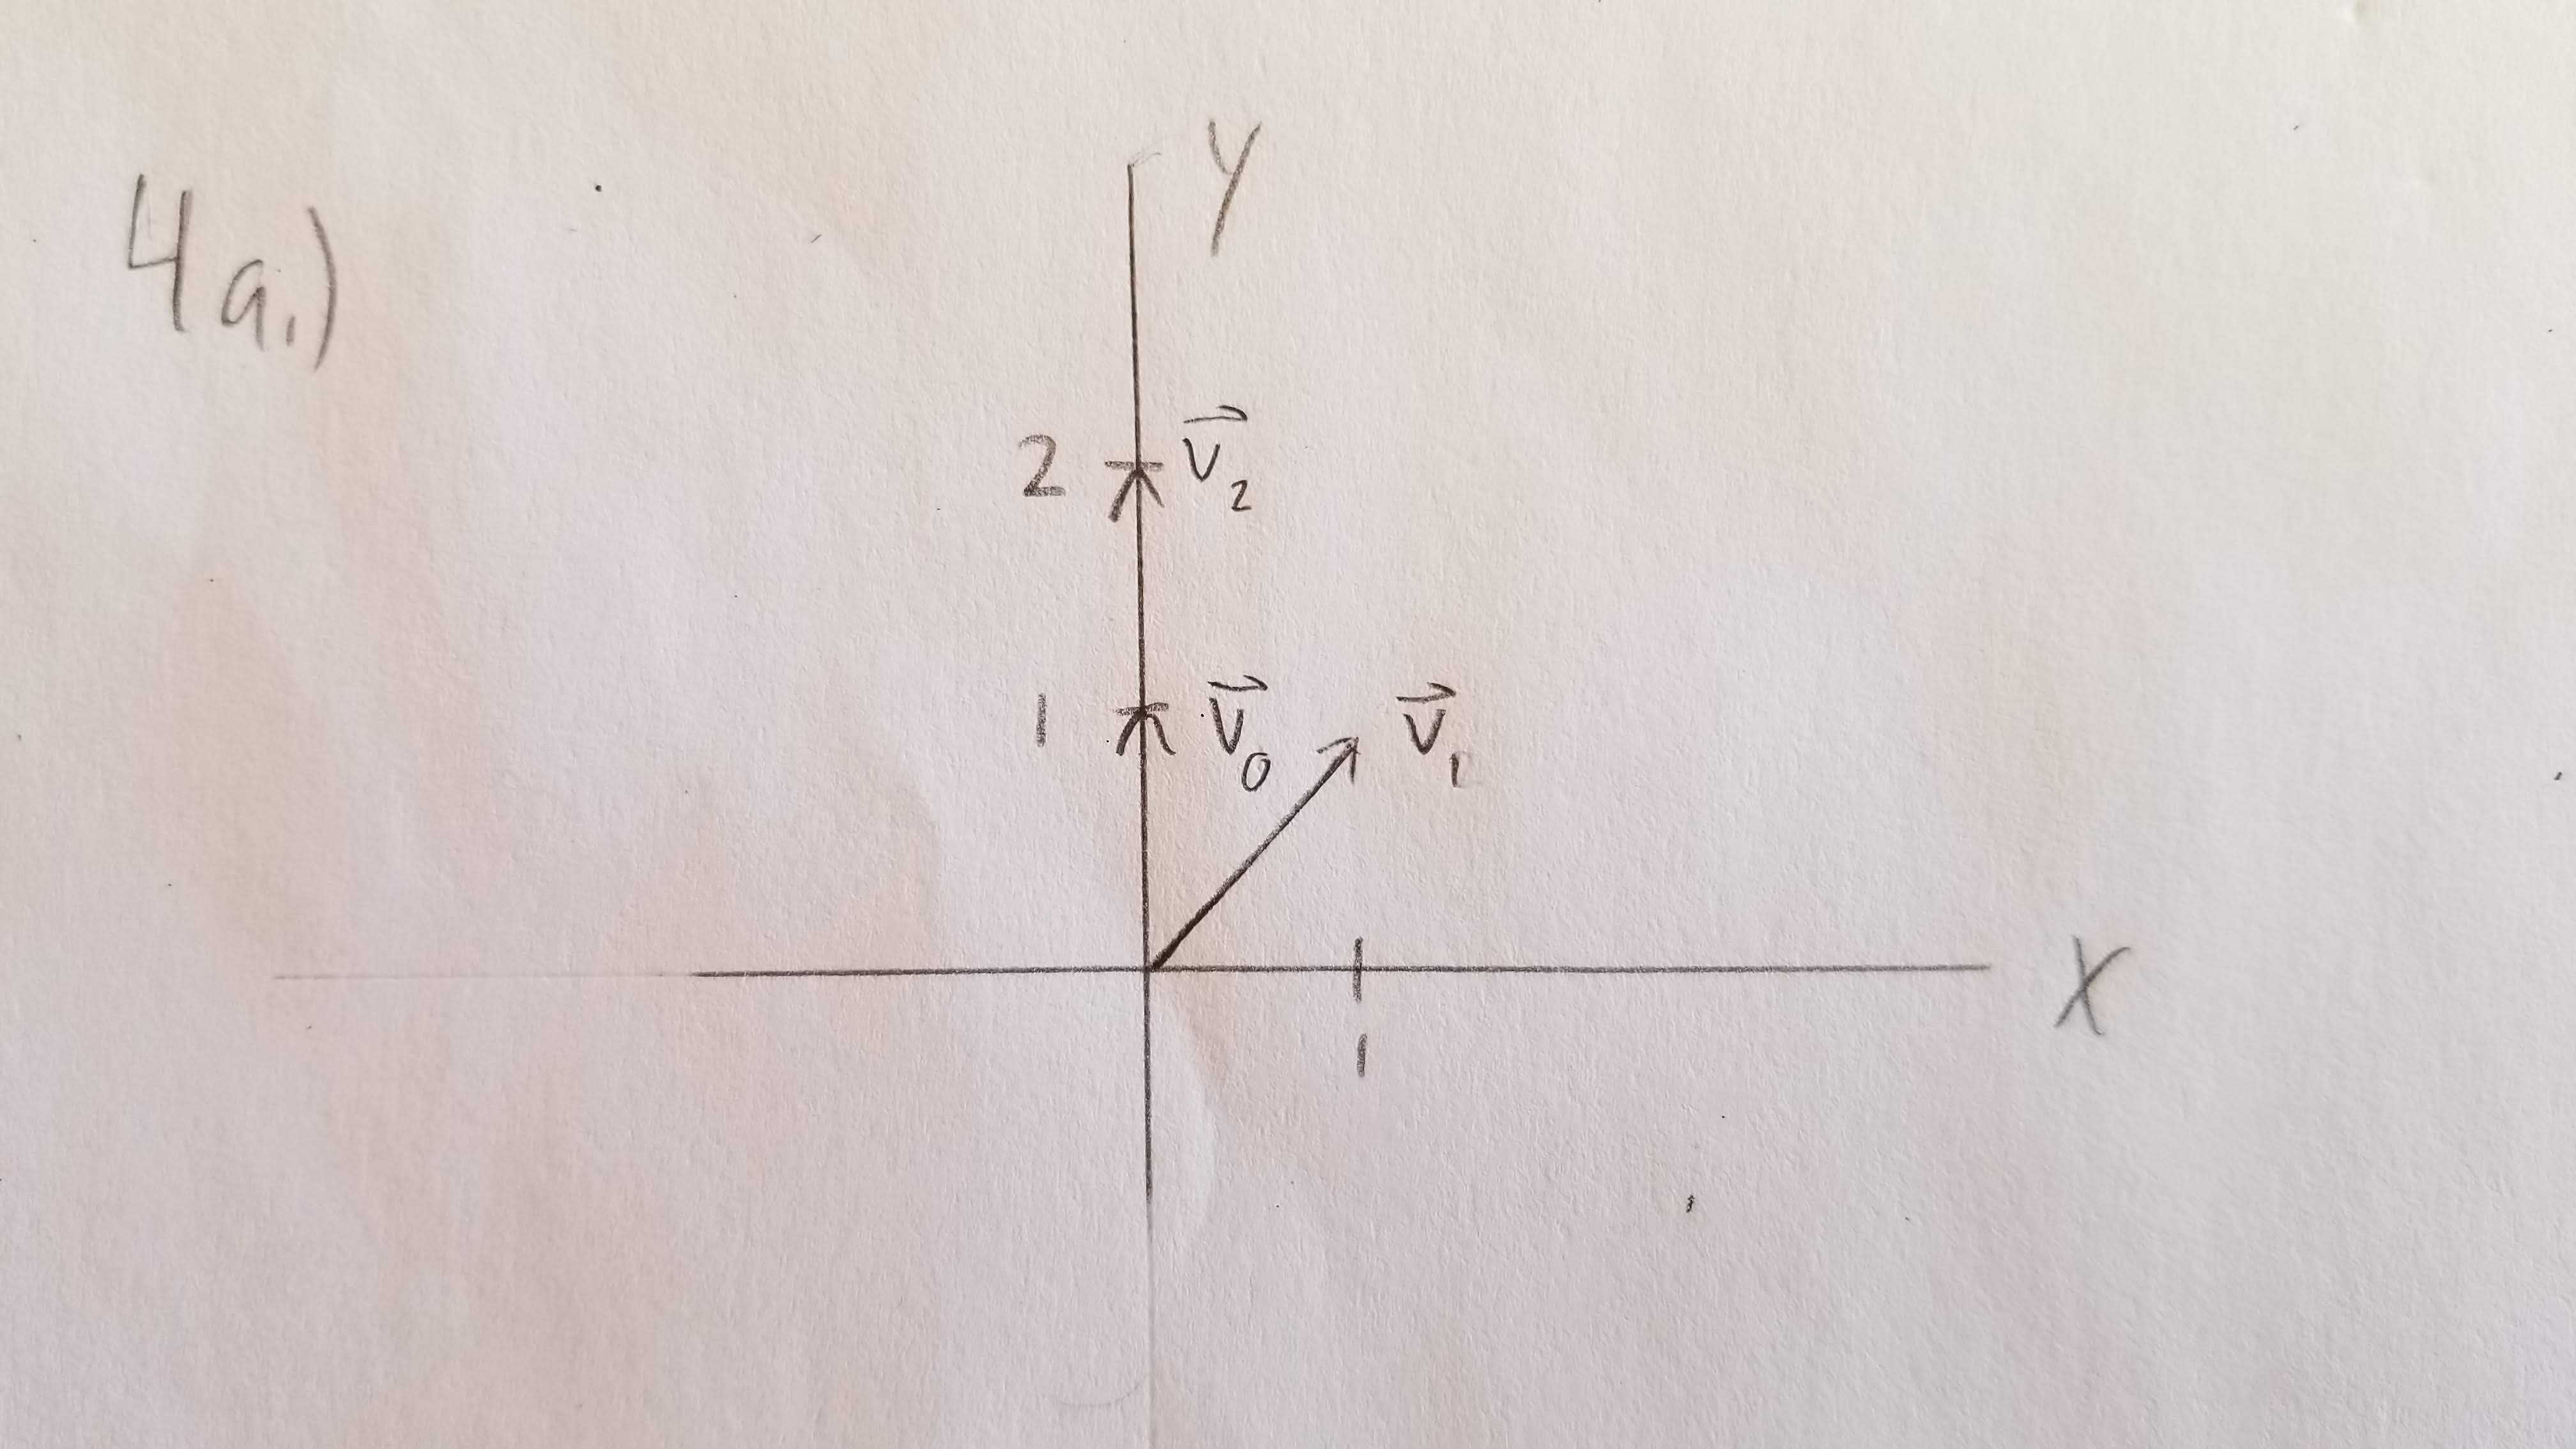
\includegraphics[width=0.7\linewidth]{20190920_153756}
\end{center}

\subsection{}

\begin{align}
	\begin{bmatrix}
	q_x \\
	q_y
	\end{bmatrix}
	&=
	\begin{bmatrix}
	\mathbf{R}_{xx} & \mathbf{R}_{xy} \\
	\mathbf{R}_{yx} & \mathbf{R}_{yy}
	\end{bmatrix}
	\begin{bmatrix}
	p_x \\
	p_y
	\end{bmatrix}
	+
	\begin{bmatrix}
	T_x \\
	T_y
	\end{bmatrix} \\
	q_x &= \mathbf{R}_{xx} p_x + \mathbf{R}_{xy} p_y + T_x \\
	q_y &= \mathbf{R}_{yx} p_x + \mathbf{R}_{yy} p_y + T_y
\end{align}
Here, \(\mathbf{q,v}\) are known, while \(\mathbf{R,T}\) are unknown. This means there are 6 unknown values with 2 equations. At minimum, 6 equations are required to find a unique solution. Since each point has 2 coordinates (i.e. \(p,q\)), a total of 6 equations is required at minimum for a unique solutions, with 3 pairs of points. 

\subsection{}

If we take 3 measurements, we obtain the following system of equations:
\begin{align}
	q_{x1} &= \mathbf{R}_{xx} p_{x1} + \mathbf{R}_{xy} p_{y1} + T_x \\
	q_{y1} &= \mathbf{R}_{yx} p_{x1} + \mathbf{R}_{yy} p_{y1} + T_y \\
	q_{x2} &= \mathbf{R}_{xx} p_{x2} + \mathbf{R}_{xy} p_{y2} + T_x \\
	q_{y2} &= \mathbf{R}_{yx} p_{x2} + \mathbf{R}_{yy} p_{y2} + T_y \\
	q_{x3} &= \mathbf{R}_{xx} p_{x3} + \mathbf{R}_{xy} p_{y3} + T_x \\
	q_{y3} &= \mathbf{R}_{yx} p_{x3} + \mathbf{R}_{yy} p_{y3} + T_y
\end{align}
Our vector of unknowns is 
\begin{equation}
	\begin{bmatrix}
	\mathbf{R}_{xx} \\
	\mathbf{R}_{xy} \\
	\mathbf{R}_{yx} \\
	\mathbf{R}_{yy} \\
	T_x \\
	T_y
	\end{bmatrix}
\end{equation}
With this information, we can convert the above set of measurements into a system of equations: 
\begin{equation}
	\begin{bmatrix}
	p_{x1} & p_{y1} & 0 & 0 & 1 & 0 \\
	0 & 0 & p_{x1} & p_{y1} & 0 & 1 \\
	p_{x2} & p_{y2} & 0 & 0 & 1 & 0 \\
	0 & 0 & p_{x2} & p_{y2} & 0 & 1 \\
	p_{x3} & p_{y3} & 0 & 0 & 1 & 0 \\
	0 & 0 & p_{x3} & p_{y3} & 0 & 1
	\end{bmatrix}
	\begin{bmatrix}
	\mathbf{R}_{xx} \\
	\mathbf{R}_{xy} \\
	\mathbf{R}_{yx} \\
	\mathbf{R}_{yy} \\
	T_x \\
	T_y
	\end{bmatrix}
	=
	\begin{bmatrix}
	q_{x1} \\
	q_{y1} \\
	q_{x2} \\
	q_{y2} \\
	q_{x3} \\
	q_{y3}
	\end{bmatrix}
\end{equation}

\subsection{}

See \texttt{iPython} notebook. 

\subsection{}

Since the points are collinear, that means that the values of subsequent points are linearly dependent. As we have proven, any matrix with linearly dependent columns does not have a unique solution. As indicated in the \texttt{iPython} notebook, the cell returns a similar error. 

\section{Properties of Pump Systems}

\subsection{}

Given the pump system as given, we can write the state steps as
\begin{align}
	x_a[n] + x_b[n] &= x_a[n + 1] \\
	0 &= x_b[n + 1]
\end{align}

\subsection{}

The transition matrix for the system is
\begin{equation}
	\mathbf{A} = 
	\begin{bmatrix}
	1 & 1 \\
	0 & 0
	\end{bmatrix}
\end{equation}

\subsection{}

Computing the results of both initial conditions,
\begin{align}
	\begin{bmatrix}
	1 & 1 \\
	0 & 0
	\end{bmatrix}
	\begin{bmatrix}
	0.5 \\
	0.5
	\end{bmatrix}
	=
	0.5 \begin{bmatrix}
	1 \\
	0
	\end{bmatrix}
	+ 
	0.5 \begin{bmatrix}
	1 \\
	0
	\end{bmatrix}
	&=
	\begin{bmatrix}
	1 \\
	0
	\end{bmatrix} \\
	\begin{bmatrix}
	1 & 1 \\
	0 & 0
	\end{bmatrix}
	\begin{bmatrix}
	0.3 \\
	0.7
	\end{bmatrix}
	=
	0.3 \begin{bmatrix}
	1 \\
	0
	\end{bmatrix}
	+ 
	0.7 \begin{bmatrix}
	1 \\
	0
	\end{bmatrix}
	&=
	\begin{bmatrix}
	1 \\
	0
	\end{bmatrix}
\end{align}

\subsection{}

You \emph{cannot} recover \(x[0]\) because there are two initial conditions for which \(x[0]\) lead to the same \(x[1]\), making the question inconclusive. 

\subsection{}

You cannot use the resultant state of the pumps to recover the initial state. This is because since effectively all the water goes into pump \(A\), meaning that as long as the initial condition satisfies the condition that they sum to the resultant vector, it is a valid starting condition. What this tells us is that \(\mathbf{A}\) is \emph{uninvertible} and does not yield a unique solution. 

\subsection{}

The transition matrix for the system shown is 
\begin{equation}
	\mathbf{A} = 
	\begin{bmatrix}
	0 & 0 & 0 \\
	0.4 & 0.5 & 0.2 \\
	0 & 0.6 & 0.35
	\end{bmatrix}
\end{equation}
The sum of the column entries is \(0.4, 1.1, 0.55\). If we subtract each pump's inputs from its outputs, we can find the net change per timestep:
\begin{align}
		\Delta P_1 &= -0.4 \\
		\Delta P_2 &= 0 \\
		\Delta P_3 &= 0.4
\end{align}
Summing up the net changes tells us that the net change in the entire system is 0, telling us that this transition matrix is \emph{conservative}. 
\section{Homework Process and Study Group}

I did this homework by myself. 

\newpage


\includepdf[pages=-]{prob3.pdf}

\end{document}
